%%%%%%%%%%%%%%%%%%%%%%%%%%%%%%%%%%%%%%%%%%%%%%%%%%%%%%%%%%%%%%%%%%%%%%%%%%%%%
%
%  System        : 
%  Module        : 
%  Object Name   : $RCSfile$
%  Revision      : $Revision$
%  Date          : $Date$
%  Author        : $Author$
%  Created By    : Robert Heller
%  Created       : 2026-11-18 09:04:58
%  Last Modified : <261118.1613>
%
%  Description 
%
%  Notes
%
%  History
% 
%%%%%%%%%%%%%%%%%%%%%%%%%%%%%%%%%%%%%%%%%%%%%%%%%%%%%%%%%%%%%%%%%%%%%%%%%%%%%
%
%    Copyright (C) 2026  Robert Heller D/B/A Deepwoods Software
%			51 Locke Hill Road
%			Wendell, MA 01379-9728
%
%    This program is free software; you can redistribute it and/or modify
%    it under the terms of the GNU General Public License as published by
%    the Free Software Foundation; either version 2 of the License, or
%    (at your option) any later version.
%
%    This program is distributed in the hope that it will be useful,
%    but WITHOUT ANY WARRANTY; without even the implied warranty of
%    MERCHANTABILITY or FITNESS FOR A PARTICULAR PURPOSE.  See the
%    GNU General Public License for more details.
%
%    You should have received a copy of the GNU General Public License
%    along with this program; if not, write to the Free Software
%    Foundation, Inc., 675 Mass Ave, Cambridge, MA 02139, USA.
%
% 
%
%%%%%%%%%%%%%%%%%%%%%%%%%%%%%%%%%%%%%%%%%%%%%%%%%%%%%%%%%%%%%%%%%%%%%%%%%%%%%



\documentclass[aspectratio=169]{beamer}

\mode<presentation>
{
  \usetheme{AnnArbor}
}
\usepackage[english]{babel}

\usepackage[latin1]{inputenc}

\usepackage{times}
\usepackage[T1]{fontenc}
\usepackage{url}
\usepackage{listings}
\lstset{language=Python,basicstyle=\footnotesize}
\usepackage{graphicx}
\title{What is Linux and Why You Should Consider Using It}
\author{Robert Heller}
\date{Wendell Resilience Hub}

%\subject{Video Presentation}

\usepackage{rphpartpage}
\setbeamertemplate{part page}[video]
\AtBeginPart{\frame{\partpage}}
\begin{document}

\frame{\titlepage}

\section{Who I am}
\begin{frame}[fragile]{Who I am}
My name is Robert Heller.  I have been using and Administrating Linux 
systems since the mid 1990s. 
\end{frame}

\section{What is Linux?}

\begin{frame}[fragile]{What Linux is}

    \begin{itemize}
        \item
            A POSIX compliant operating system kernel,
        \pause 
        \item
            Created by Linus Torvalds as a ``hobby project'' in 1994.
        \pause
        \item
            It is now the operating system kernel for almost all of the 
            World Wide Web.
        \pause
        \item
            Used in all super computers,
        \pause
        \item
            Used in most network appliances and smart phones.
    \end{itemize}
\end{frame} 

\begin{frame}[fragile]{What a modern desktop GNU/Linux distribution is}
    \begin{itemize}
        \item
            The Linux kernel.
        \pause
        \item
            The GNU core utilities: basic POSIX utilities.
        \pause
        \item
            A graphical desktop subsystem.
        \pause
        \item
            A collection of commonly useful applications
        \pause
        \item
            A software package management system with a repository of 
            software.
     \end{itemize}
\end{frame}

\section{How Linux is different from MS-Windows}

\begin{frame}[fragile]{Linux is Free}
    \begin{itemize}
        \item
            Linux is available at no cost.
        \pause
        \item
            You can run Linux on any number of computers, including 
            giving it to a friend.
        \pause
        \item
            You can run Linux for as long as you like.
        \pause
        \item
            You don't need an online account to use Linux.
    \end{itemize}
\end{frame}

\begin{frame}[fragile]{Will MS-Windows applications run on Linux}
    \begin{itemize}
        \item
            Short answer: no.
        \pause
        \item
            Longer answer: some can with some sort of helper system.
        \pause
        \item
            Some common applications have been built for Linux.
            \pause
            \begin{itemize}
                \item Firefox
                \pause
                \item Chromium / Chrome
                \pause
                \item VLC
                \pause
                \item
                    Many video games have been ported to Linux
             \end{itemize}
        \pause
        \item
            Other common applications have Open Source alternatives.
            \pause
            \begin{itemize}
                \item LibreOffice can replace MS-Office
                \pause
                \item Gimp can replace Photoshop
                \pause
                \item Inkscape can replace Illustrator
            \end{itemize}
        \pause
        \item
            Web / Cloud based applications will work.
        \pause
        \item
            There are emulators available: Wine, and others.
    \end{itemize}
\end{frame}

\begin{frame}[fragile]{Contact Information}
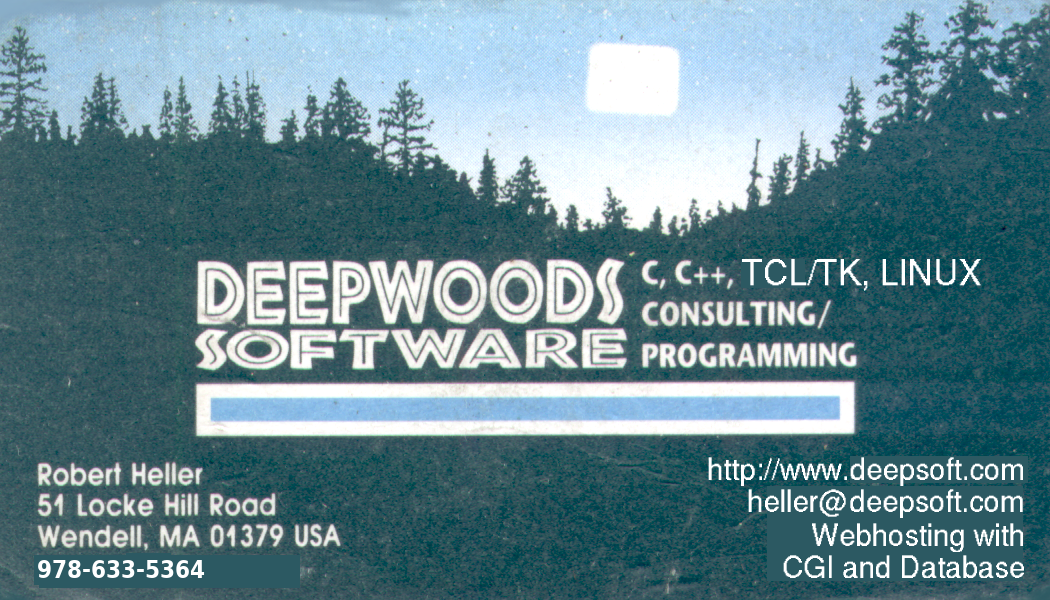
\includegraphics[height=2.75in]{NewCard.png}
\end{frame}
\end{document}
